\normalfalse \difficiletrue \tdifficilefalse
\correctionfalse

%\UPSTIidClasse{11} % 11 sup, 12 spé
%\newcommand{\UPSTIidClasse}{12}

\exer{Barrière Sympact $\star\star$ \label{B2:12:14}}
\setcounter{question}{0}\marginnote{\xpComp{CIN}{01}}%\UPSTIcompetence[2]{B2-13}
\index{Compétence B2-13-PTSI}
\index{Barrière Sympact}
\ifcorrection
\else
\marginnote{\textbf{Pas de corrigé pour cet exercice.}}
\fi
\ifprof
\else
Soit le mécanisme suivant.
\begin{marginfigure}
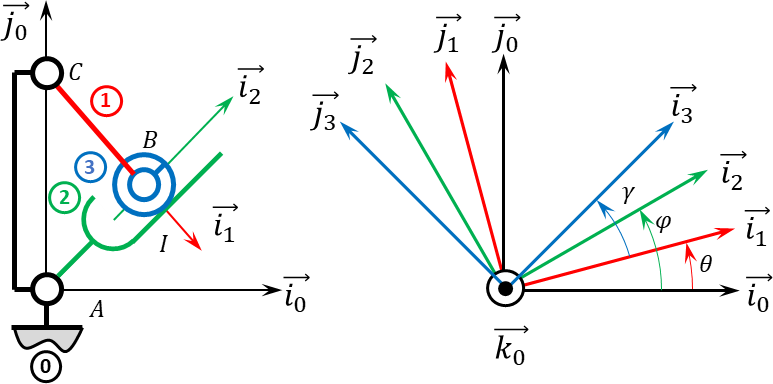
\includegraphics[width=\linewidth]{15_01}
\end{marginfigure}
\fi



\question{Réaliser le paramétrage du mécanisme.}
\ifprof
\else
\fi


\ifprof
\else
\marginnote{Corrigé voir \ref{CIN:01:B2:12:14}.}

\fi